% EVIDENT (Execution-Verified Identification and Diagnosis of Evidence in Noisy Tables), ACL / ARR format (8 pages of content; references, Limitations and appendices are outside the limit).
% Working draft: red [TODO] boxes mark results that are not yet measured. They must all be gone before submission.
% Build: pdflatex evident_acl && bibtex evident_acl && pdflatex evident_acl && pdflatex evident_acl
% Every number in the text is a macro generated by evident/eval/make_paper_tables.py (run build_tables.sh); do not type numbers by hand.
\documentclass[11pt]{article}
\usepackage[review]{acl}   % anonymous review version; "final" for camera-ready
\usepackage{times}
\usepackage{latexsym}
\usepackage[T1]{fontenc}
\usepackage[utf8]{inputenc}
\usepackage{microtype}
\usepackage{inconsolata}
\usepackage{graphicx,booktabs,multirow,amsmath,amssymb,xcolor,enumitem,array}
\usepackage{tikz}
\usetikzlibrary{positioning,arrows.meta,fit,backgrounds,calc}
\setlist{nosep,leftmargin=*}
\newcolumntype{R}[1]{>{\raggedright\arraybackslash}p{#1}}

\newif\ifdraft \drafttrue   % \draftfalse hides TODO boxes
\newcommand{\todo}[1]{\ifdraft\textcolor{red}{\textbf{[TODO: #1]}}\fi}
\newcommand{\benchmark}{\mbox{EVIDENT}}  % Execution-Verified Identification and Diagnosis of Evidence in Noisy Tables (2026-10-31; replaces REXA-DB, DREDGE, DERIVE)
% AUTO-GENERATED by eval/make_paper_tables.py from reports/eval_final_v6. Do not edit.
\newcommand{\orValueP}{74\%}
\newcommand{\bmValueZeroP}{68\%}
\newcommand{\bmValueTopP}{40\%}
\newcommand{\bmMissedTableP}{37\%}
\newcommand{\bmMissedZeroP}{10\%}
\newcommand{\bmMissedTopP}{51\%}
\newcommand{\fsCiPoints}{95\% CI $-1$ to $+5$ points}
\newcommand{\rrSuffP}{75\%}
\newcommand{\rrNotSuffP}{2\%}
\newcommand{\nQuestions}{200}
\newcommand{\topLevel}{500}
\newcommand{\nLevels}{6}
\newcommand{\nPredictions}{1200}
\newcommand{\bmValueZero}{0.680}
\newcommand{\bmValueTop}{0.400}
\newcommand{\bmDeltaTop}{-28.0 points (95\% CI -35.8 to -19.7)}
\newcommand{\bmDeltaAbsTop}{28.0}
\newcommand{\bmDeltaHundred}{-26.5 points (95\% CI -33.7 to -19.5)}
\newcommand{\fsDeltaTop}{+1.5 points; 95\% CI -1.2 to +4.7}
\newcommand{\fsDeltaMid}{-3.0 points; 95\% CI -6.9 to +1.6}
\newcommand{\orDeltaTop}{+0.0 points (95\% CI -2.1 to +2.0)}
\newcommand{\bmValue}{0.498}
\newcommand{\fsValue}{0.713}
\newcommand{\orValue}{0.743}
\newcommand{\rrValue}{0.206}
\newcommand{\rrValueZero}{0.310}
\newcommand{\bmValueAtZero}{0.680}
\newcommand{\bmRecallZero}{0.997}
\newcommand{\bmRecallTop}{0.665}
\newcommand{\qbRecallZero}{0.993}
\newcommand{\qbRecallTop}{0.000}
\newcommand{\bmSuffZero}{0.764}
\newcommand{\bmSuffTop}{0.500}
\newcommand{\bmMissedTable}{36.9\%}
\newcommand{\fsTokZero}{924}
\newcommand{\fsTokTop}{53{,}190}
\newcommand{\bmTokTop}{712}
\newcommand{\tokRatioTop}{75}
\newcommand{\orBird}{0.623}
\newcommand{\orSpider}{0.863}
\newcommand{\orNested}{0.601}
\newcommand{\orLookup}{1.000}
\newcommand{\nFourTables}{26}
\newcommand{\orTOne}{0.862}
\newcommand{\orTFour}{0.372}
\newcommand{\fsTOne}{0.812}
\newcommand{\fsTFour}{0.474}
\newcommand{\bmTOne}{0.721}
\newcommand{\bmTFour}{0.192}
\newcommand{\setGainMin}{2.7}
\newcommand{\setGainMax}{4.5}
\newcommand{\orSetBird}{0.665}
\newcommand{\bmSetDeltaPts}{-28.5}
\newcommand{\bmCorrectInsuff}{7.4\%}
\newcommand{\bmCorrectInsuffEq}{3.8\%}
\newcommand{\bmWrongSuff}{11.7\%}
\newcommand{\fsCorrectInsuff}{3.3\%}
\newcommand{\fsCorrectInsuffEq}{1.0\%}
\newcommand{\fsWrongSuff}{15.4\%}
\newcommand{\orCorrectInsuff}{4.8\%}
\newcommand{\orCorrectInsuffEq}{0.7\%}
\newcommand{\orWrongSuff}{15.3\%}
\newcommand{\rrSuffAcc}{0.750}
\newcommand{\rrSuffN}{80}
\newcommand{\rrNotSuffAcc}{0.017}
\newcommand{\rrNotSuffN}{120}
\newcommand{\rrBigAccPct}{2.9\%}
\newcommand{\rrBigSuffPct}{2.9\%}
\newcommand{\bmBigAccPct}{47.8\%}
\newcommand{\rrBigN}{69}
\newcommand{\rrBigAcc}{0.029}
\newcommand{\rrBigSuff}{0.029}
\newcommand{\bmBigAcc}{0.478}
\newcommand{\rrSmallAccPct}{52.3\%}
\newcommand{\rrSmallSuffPct}{67.3\%}
\newcommand{\rrSuffAccPct}{75.0\%}
\newcommand{\rrNotSuffAccPct}{1.7\%}
\newcommand{\rrSmallN}{107}
\newcommand{\rrSmallAcc}{0.523}
\newcommand{\rrSmallSuff}{0.673}
\newcommand{\bmRowsSmallAcc}{0.804}
\newcommand{\bmRowsHugeAcc}{0.419}
\newcommand{\nCompleteSet}{147}
\newcommand{\nOverFiveThousand}{22}
\newcommand{\nOverNinety}{69}
\newcommand{\orLatZero}{3.0}
\newcommand{\orLatTop}{42.3}
\newcommand{\orFlips}{7}
\newcommand{\nSysErr}{0}
\newcommand{\nSysErrSystems}{none}
\newcommand{\gpOrValue}{0.695}
\newcommand{\gpOrDelta}{+0.5 points; 95\% CI +0.0 to +1.6}
\newcommand{\gpFsValue}{0.681}
\newcommand{\gpFsDelta}{-1.5 points; 95\% CI -5.9 to +3.3}
\newcommand{\gpBmValue}{0.532}
\newcommand{\gpBmDelta}{-25.0 points; 95\% CI -32.7 to -17.6}
\newcommand{\gmOrValueCommon}{0.743}
\newcommand{\gpDiffOr}{-4.8 points; 95\% CI -9.3 to -1.0}
\newcommand{\gpDiffOrSig}{significant}
\newcommand{\gmFsValueCommon}{0.716}
\newcommand{\gpDiffFs}{-3.5 points; 95\% CI -7.5 to +1.3}
\newcommand{\gpDiffFsSig}{not significant}
\newcommand{\gmBmValueCommon}{0.539}
\newcommand{\gpDiffBm}{-0.6 points; 95\% CI -4.5 to +3.5}
\newcommand{\gpDiffBmSig}{not significant}
\newcommand{\gpBmDeltaAbs}{25.0}
\newcommand{\gpBmRefusals}{2.9\%}
\newcommand{\gmOrSuffCommon}{0.844}
\newcommand{\gmOrExecCommon}{0.721}
\newcommand{\gmOrZeroCommon}{0.745}
\newcommand{\gmOrTopCommon}{0.750}
\newcommand{\gmFsSuffCommon}{0.837}
\newcommand{\gmFsExecCommon}{0.704}
\newcommand{\gmFsZeroCommon}{0.715}
\newcommand{\gmFsTopCommon}{0.705}
\newcommand{\gmBmSuffCommon}{0.626}
\newcommand{\gmBmExecCommon}{0.525}
\newcommand{\gmBmZeroCommon}{0.680}
\newcommand{\gmBmTopCommon}{0.415}
\newcommand{\gmBmMissedCommon}{30.4\%}
\newcommand{\gmFsTokCommonTop}{12{,}427}
\newcommand{\gmBmMissedZeroP}{10\%}
\newcommand{\gmBmMissedCommonTopP}{46\%}
\newcommand{\gpOrSuffCommon}{0.848}
\newcommand{\gpOrExecCommon}{0.676}
\newcommand{\gpOrZeroCommon}{0.695}
\newcommand{\gpOrTopCommon}{0.700}
\newcommand{\gpFsSuffCommon}{0.830}
\newcommand{\gpFsExecCommon}{0.660}
\newcommand{\gpFsZeroCommon}{0.690}
\newcommand{\gpFsTopCommon}{0.675}
\newcommand{\gpBmSuffCommon}{0.676}
\newcommand{\gpBmExecCommon}{0.509}
\newcommand{\gpBmZeroCommon}{0.675}
\newcommand{\gpBmTopCommon}{0.425}
\newcommand{\gpBmMissedCommon}{29.4\%}
\newcommand{\gpFsTokCommonTop}{12{,}427}
\newcommand{\gpBmMissedZeroP}{12\%}
\newcommand{\gpBmMissedCommonTopP}{40\%}
\newcommand{\gpNPredictions}{2{,}400}
\newcommand{\gpCommonTop}{100}
\newcommand{\gpSameOrder}{identically}
\newcommand{\gpPatternHolds}{holds}
\newcommand{\bmDevZero}{0.613}
\newcommand{\bmDevTop}{0.349}
\newcommand{\bmDevDelta}{-26.4}
\newcommand{\fsDevZero}{0.708}
\newcommand{\fsDevTop}{0.708}
\newcommand{\fsDevDelta}{+0.0}
\newcommand{\orDevZero}{0.708}
\newcommand{\orDevTop}{0.726}
\newcommand{\orDevDelta}{+1.9}
\newcommand{\nDevDb}{15}
\newcommand{\nDevQ}{106}
\newcommand{\bmTestZero}{0.755}
\newcommand{\bmTestTop}{0.457}
\newcommand{\bmTestDelta}{-29.8}
\newcommand{\fsTestZero}{0.723}
\newcommand{\fsTestTop}{0.755}
\newcommand{\fsTestDelta}{+3.2}
\newcommand{\orTestZero}{0.787}
\newcommand{\orTestTop}{0.766}
\newcommand{\orTestDelta}{-2.1}
\newcommand{\nTestDb}{16}
\newcommand{\nTestQ}{94}
\newcommand{\bmDbDecline}{23}
\newcommand{\bmDbSame}{7}
\newcommand{\bmDbImprove}{1}
\newcommand{\bmLodoMin}{-29.8}
\newcommand{\bmLodoMax}{-26.7}
\newcommand{\bmSignP}{$1.5\times10^{-6}$}
\newcommand{\fsDbDecline}{2}
\newcommand{\fsDbSame}{25}
\newcommand{\fsDbImprove}{4}
\newcommand{\fsLodoMin}{+0.5}
\newcommand{\fsLodoMax}{+2.2}
\newcommand{\fsSignP}{0.89}
\newcommand{\nSqlPredictions}{6{,}000}
\newcommand{\nValueOnly}{108}
\newcommand{\nValueColOrder}{107}
\newcommand{\nValueAccidental}{1}
\newcommand{\nProbeTrials}{1{,}200}
\newcommand{\nProbeChanged}{0}
\newcommand{\bmMissedTenP}{26\%}
\newcommand{\bmMissedFiftyP}{38\%}
\newcommand{\bmMissedHundredP}{46\%}
\newcommand{\bmMissedTwoFiftyP}{49\%}
\newcommand{\bmMissedFiveHundredP}{51\%}
\newcommand{\bmShownZero}{0.951}
\newcommand{\bmShownHundred}{0.667}
\newcommand{\bmShownTop}{0.595}
\newcommand{\orExec}{0.723}
\newcommand{\fsExec}{0.699}
\newcommand{\bmExec}{0.486}
\newcommand{\bmMissedOfWrongP}{72\%}
\newcommand{\nOpAggregate}{50}
\newcommand{\nOpFilter}{15}
\newcommand{\nOpGroup}{46}
\newcommand{\nOpJoin}{39}
\newcommand{\nOpNested}{43}
\newcommand{\nOpLookup}{7}
\newcommand{\nFourBird}{20}
\newcommand{\nCandZeroMax}{13}
\newcommand{\nCandTopMax}{513}
\newcommand{\orBirdTOne}{0.735}
\newcommand{\orBirdTFour}{0.458}
\newcommand{\bmBirdTOne}{0.623}
\newcommand{\bmBirdTFour}{0.250}
\newcommand{\nAltReviewed}{33}
\newcommand{\nAltConfirmed}{25}
\newcommand{\nMissedHandChecked}{93}
\newcommand{\nMissedHandConfirmed}{93}
\newcommand{\nOrShortcutCases}{7}
\newcommand{\nOrShortcutValid}{6}
\newcommand{\probeAucBird}{0.62}
\newcommand{\probeAucAll}{0.53}
\newcommand{\tokSqlRunM}{22.2}
\newcommand{\tokSqlFsShareP}{93\%}
\newcommand{\tokRrRunM}{2.1}
\newcommand{\tokGpRunM}{5.6}


\title{Is the Evidence Behind Relational Answers Sufficient\\
as the Search Space Grows?}
\author{Anonymous ACL submission}

\begin{document}
\maketitle

\begin{abstract}
Relational question answering is increasingly posed over warehouses without saying which tables matter. A correct answer then requires discovering \emph{sufficient} evidence (tables, columns, join keys, and every qualifying row) among many irrelevant candidates, yet current benchmarks cannot tell whether a system failed to find that evidence or misused it. To test whether the evidence behind an answer is sufficient as the search space grows, we introduce \benchmark, a benchmark that (i) holds BIRD and Spider questions, data, and answers fixed while adding nested sets of up to \topLevel{} real, irrelevant tables; (ii) releases executable gold evidence at table, column, join-key, and row level, verified to reproduce every answer; and (iii) scores any system, SQL-writing or not, on answer correctness, evidence relevance and sufficiency, and the pipeline stage that failed. In a \nQuestions-question pilot, irrelevant tables cost a BM25 schema-retrieval pipeline \bmDeltaAbsTop{} accuracy points with Gemini 2.5 Flash (\gpBmDeltaAbs{} with GPT-4o at +\gpCommonTop{} tables), and evidence-level scoring traces the loss to discovery: predictions whose prompt lacks a required table rise from \bmMissedZeroP{} to \bmMissedTopP{}. Showing every schema is unaffected but costs \tokRatioTop{} times the input tokens, and a reader without SQL is bounded by the rows it can retrieve and fit.
\end{abstract}

\section{Introduction}\label{sec:intro}
Language models are now asked questions about organizational data directly: an analyst types ``which supplier had the highest total sales last year?'' into an assistant connected to a warehouse with hundreds of tables. Before any query is written, the system must decide which tables, columns, and join paths are relevant, and the answer is trustworthy only if the evidence behind it is \emph{sufficient}. One missed join key, one table of returns left out, or one omitted qualifying record changes the result, however fluent the answer or well-formed the query. In this setting, the decisive step is often not writing SQL but \emph{finding the evidence}.

Current evaluation does not isolate that step. Text-to-SQL benchmarks such as BIRD and Spider \citep{bird,spider} give each question its own database, typically a handful of tables, and score a single execution result. A wrong answer may come from choosing the wrong table, missing a join, reading too few rows, or misreasoning over the right evidence; accuracy merges all four. Multi-table benchmarks scale the serialized context of small databases \citep{tqabench}, retrieve among web tables without relational schema \citep{trag}, or template questions over fixed corpora \citep{mmqa}. In natural collections, larger databases also come with different and harder questions, so the effect of the search space cannot be separated from the effect of the question. Finally, table recall measures \emph{relevance}, not \emph{sufficiency}: a system can retrieve every relevant table and still fail because it read 30 of 400 qualifying rows.

Our question is therefore the one in the title: \emph{is the evidence behind an answer sufficient, and does it stay sufficient as the search space grows?} Answering it requires evaluating relational QA at the level of evidence, under a search space that is varied while everything else is held fixed. Under that protocol, the two sources of failure that accuracy merges, \emph{not finding} the evidence and \emph{not using} it correctly, can be separated, and the separation changes the conclusions drawn about systems. We introduce \benchmark{} (\textbf{E}xecution-\textbf{V}erified \textbf{I}dentification and \textbf{D}iagnosis of \textbf{E}vidence in \textbf{N}oisy \textbf{T}ables), a benchmark that implements this protocol through three design choices (Figure~\ref{fig:overview}):
\begin{itemize}
\item \textbf{Controlled search space.} Each natural BIRD or Spider question keeps its database, data, and gold answer, while nested sets of 10 to \topLevel{} real tables from unrelated databases are added. Any change in behavior is caused by the candidates, not by the question.
\item \textbf{Executable gold evidence.} For every question we release the required tables, columns, join keys, and rows, including the \emph{complete qualifying set} for aggregation, ranking, and negation. A database built from the evidence alone must reproduce the gold answer, so sufficiency can be tested by execution rather than judged.
\item \textbf{Method-agnostic scoring.} Systems return whatever they produce (an answer, SQL, selected tables, retrieved rows). The scorer reports answer correctness, evidence relevance, evidence sufficiency, and the first pipeline stage that failed, so text-to-SQL pipelines and readers that never write SQL are measured on one scale.
\end{itemize}

A pilot of \nQuestions{} questions with two model families shows why this matters. \textbf{(1)} With no added tables, BM25 schema retrieval looks nearly as good as showing the model every schema (value accuracy \bmValueAtZero{} vs.\ \gmFsZeroCommon{}), yet with \topLevel{} added tables it loses \bmDeltaAbsTop{} points with Gemini 2.5 Flash while full-schema prompting does not move; GPT-4o, run up to +\gpCommonTop{}, shows the same pattern. \textbf{(2)} Evidence-level scoring attributes the loss: \bmMissedOfWrongP{} of the pipeline's wrong answers had a required table missing from the prompt, whereas the remaining errors of full-context systems are query planning and reasoning over evidence they had. Better retrieval would fix the former and not the latter. \textbf{(3)} Correct answers built on insufficient evidence are rare (at most \bmCorrectInsuffEq{} once equivalent derivations are accepted), so the stage labels are trustworthy. \textbf{(4)} A reader without SQL answers \rrSuffAccPct{} of questions whose retrieved rows suffice but almost none of the rest; its evidence falls short because \nOverNinety{} of \nQuestions{} questions need more qualifying rows than fit in its prompt and keyword search misses others.

\paragraph{Research questions.}
\textbf{RQ1} How does irrelevant relational context affect evidence discovery and answer correctness when the question, data, and answer are fixed?
\textbf{RQ2} How does relational complexity (tables joined, evidence volume) affect evidence selection and reasoning?
\textbf{RQ3} How do SQL-based and non-SQL paradigms acquire and use sufficient evidence, and at what token cost?
\textbf{RQ4} Can errors be attributed to evidence discovery versus evidence use?

\paragraph{Contributions.}
(1)~A controlled relational search-space benchmark: natural BIRD and Spider questions with up to \topLevel{} added real tables, size-matched and screened against look-alikes, with database-level development and held-out splits (Section~\ref{sec:design}).
(2)~Executable evidence annotations at table, column, join-key, and record level, including complete qualifying sets, with an execution-based, equivalence-aware sufficiency measure (Sections~\ref{sec:task}--\ref{sec:eval}).
(3)~A system-agnostic scorer that reports answer correctness, relevance, sufficiency, and stage-wise failure attribution.
(4)~An empirical study of retrieval-based, full-context, and non-SQL systems with two LLM families, robust across held-out databases and leave-one-database-out analysis (Section~\ref{sec:results}).
We release construction scripts, manifests, annotations, and the scorer.

\begin{table*}[t]\centering\footnotesize\setlength{\tabcolsep}{3pt}
\begin{tabular}{R{1.9cm}R{3.0cm}R{2.9cm}R{2.2cm}R{3.3cm}R{1.4cm}}\toprule
Resource & Candidate scale varied independently? & Gold evidence released & Joins / aggregation & What is scored & Failure attribution\\\midrule
BIRD, Spider & No (database given) & None at record level & Yes (gold SQL) & Execution result of one SQL query & No\\
CRUSH4SQL & No (fixed unions); budget varied & Columns of gold SQL & Yes (gold SQL) & Column recall at budget; downstream EM/EX & No\\
DBCopilot & No (fixed collections: 876 / 597 / 152 tables) & Database and tables of gold SQL & Yes (gold SQL) & Database/table Recall@$k$, mAP; EX; cost & No\\
TQA-Bench & No (2--6 tables per database) & Not reported & Yes & Answer accuracy over serialized tables & No\\
T-RAG / MultiTableQA & Fixed corpora & Source-table label & No SQL or keys & Table retrieval recall, latency & No\\
MMQA & No size variation found & Tables, keys; no rows & Yes (templates) & Retrieval P/R/F1, SQL ROUGE/BLEU, keys & No\\
MT-RAIG & No (fixed 19{,}563-table corpus); top-$k$ varied & Gold table sets (2.9 per question) & Joinable tables; no SQL & Table R@$k$; LLM-judged faithfulness, completeness & No\\
TANQ & Open-domain corpus & Cell-level attribution & Aggregation; no relational DB & Answer table, cell attribution & Attribution only\\
WTQ, HiTab, AIT-QA & No (one table given) & HiTab only (linked cells) & No joins & Answer match & No\\
\midrule
\textbf{\benchmark{} (ours)} & \textbf{Yes (nested decoys)} & \textbf{Tables, columns, joins, rows; executable} & \textbf{Yes} & \textbf{Answer, relevance, sufficiency; SQL or not} & \textbf{Yes (by stage)}\\\bottomrule
\end{tabular}
\caption{Property comparison; entries come from the papers and released data (``What is scored'' lists the main metrics each paper reports).}\label{tab:coverage}
\end{table*}

\section{Related Work}\label{sec:related}
\paragraph{Text-to-SQL and schema scale.} BIRD stresses real database content, external knowledge, and efficiency \citep{bird}; Spider tests cross-database generalization \citep{spider}. Both give the system its database (BIRD development databases hold 3--14 tables, Spider's up to 26) and score the result of one query. Neither releases record-level evidence, so a right answer from insufficient evidence is indistinguishable from a sound one. Closest to our setting, CRUSH4SQL merges the 166 Spider schemas into one collection of 876 tables (SpiderUnion; BirdUnion merges BIRD's 11 development schemas into 75 tables), retrieves a schema subset by having an LLM hallucinate a minimal schema, and scores column recall at a fixed retrieval budget and downstream execution accuracy \citep{crush4sql}. DBCopilot routes questions to a database and tables within fixed collections built the same way (876, 597, and 152 tables for Spider, BIRD, and Fiben) and reports Recall@$k$, mAP, execution accuracy, and cost \citep{dbcopilot}. Others argue that long-context models can take the full schema \citep{longctxsql}, and Spider~2.0 poses enterprise workflows over very large schemas \citep{spider2}. These works propose \emph{systems} and evaluate them on one fixed collection per dataset; what they vary is the retrieval budget, not the collection. CRUSH4SQL's observation that SQL accuracy drops once more than 30 retrieved columns enter the prompt is an early sign of the distraction effect we isolate. \benchmark{} varies the collection size for fixed questions, which turns ``does the method scale?'' into a measurable curve, and scores the evidence behind each answer, not only the schema subset or execution result; schema-routing systems such as DBCopilot are natural systems to evaluate on it. We reuse BIRD and Spider questions so that ability is not confounded with newly written ones.

\paragraph{Multi-table QA and table retrieval.} TQA-Bench scales the serialized context of 2--6 table databases to 8K--64K tokens \citep{tqabench}; it varies context length, whereas we vary the number of candidate tables with the relevant database unchanged. MMQA builds 5{,}000 two- and three-table questions on Spider from 45 SQL templates and evaluates table retrieval, SQL (ROUGE/BLEU), and key selection; we found no experiment varying its corpus size \citep{mmqa}. T-RAG retrieves among 60K web tables without relational schema and reports recall and latency \citep{trag}. MT-RAIG asks for insights over multiple unknown tables, retrieving from a corpus of 19{,}563 tables built from joinable Spider and Open-WikiTable tables, and scores table Recall@$k$ and LLM-judged faithfulness and completeness of long-form insights; it varies the number of retrieved tables but not the corpus, and its answers are not executable \citep{mtraig}. To our knowledge none of these combines controlled candidate growth, executable evidence beyond the relevant table, and method-agnostic scoring (Table~\ref{tab:coverage}); we do not claim to have surveyed all schema-linking work.

\paragraph{Evidence, attribution, and distraction.} Attribution evaluation asks whether generated text is supported by identified sources \citep{ais,alce}. In tables, HiTab links answers to cells of a single table \citep{hitab} and TANQ attributes every cell of table-valued answers to open-domain sources \citep{tanq}; WTQ and AIT-QA give each question its one table \citep{wtq,aitqa}. Beyond relational data, OTT-QA retrieves evidence from over 400K Wikipedia tables and linked passages for multi-hop open-domain questions \citep{ottqa}, and MultiHiertt annotates supporting facts for numerical reasoning over multiple hierarchical tables and text in financial reports \citep{multihiertt}; both score answers with exact match and F1 and neither involves joins or executable queries. Our evidence spans tables and join keys, covers complete qualifying sets, and is verified by execution, which lets us ask whether evidence is \emph{enough}, not only whether it is related. LLMs are known to be distracted by irrelevant context \citep{distracted} and to use long contexts unevenly \citep{lostmiddle}; \benchmark{} measures the relational analogue, irrelevant tables, with the answer held fixed.

\begin{figure*}[t]\centering
\resizebox{\textwidth}{!}{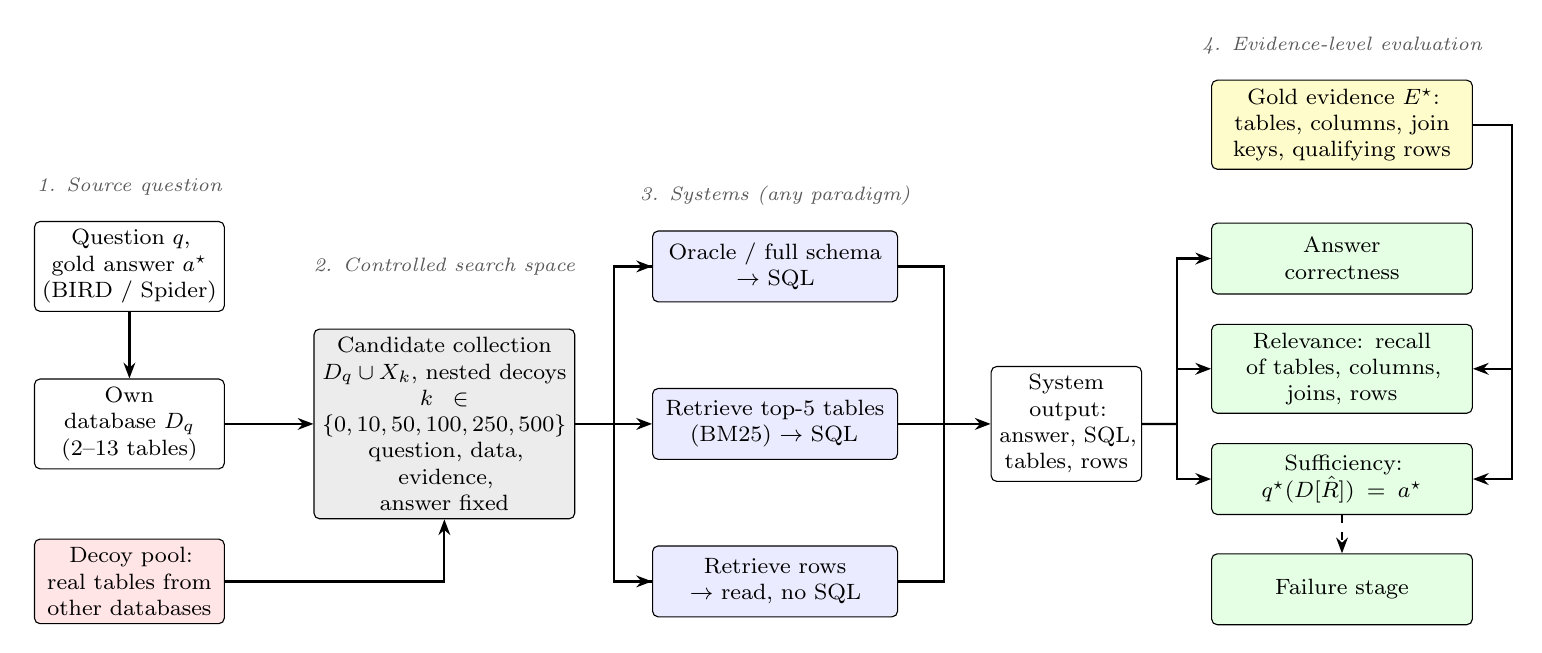
\begin{tikzpicture}[font=\footnotesize,
  box/.style={draw, rounded corners=2pt, align=center, inner sep=3pt, minimum height=9mm, fill=white},
  gold/.style={box, fill=yellow!20, text width=31mm},
  sys/.style={box, fill=blue!8, text width=29mm},
  met/.style={box, fill=green!10, text width=31mm},
  lab/.style={font=\scriptsize\itshape, text=black!65},
  arr/.style={-{Stealth[length=2mm]}, thick},
  bus/.style={thick}]
% columns (cm): 0 source | 4.0 candidates | 8.2 systems | 11.9 output | 15.4 evaluation
\node[box, text width=22mm] (q)   at (0,3.2)  {Question $q$,\\ gold answer $a^\star$\\ (BIRD / Spider)};
\node[box, text width=22mm] (own) at (0,1.2)  {Own database $D_q$\\ (2--13 tables)};
\node[box, text width=22mm, fill=red!10] (dec) at (0,-0.8) {Decoy pool: real tables from other databases};
\node[box, text width=31mm, fill=gray!15] (cand) at (4.0,1.2) {Candidate collection\\ $D_q \cup X_k$, nested decoys\\ $k\in\{0,10,50,100,250,500\}$\\ question, data, evidence,\\ answer fixed};
% when dense / hybrid / graph retrievers are evaluated, list them in s2 again
\node[sys] (s1) at (8.2,3.2)  {Oracle / full schema\\ $\rightarrow$ SQL};
\node[sys] (s2) at (8.2,1.2)  {Retrieve top-5 tables (BM25) $\rightarrow$ SQL};
\node[sys] (s3) at (8.2,-0.8) {Retrieve rows\\ $\rightarrow$ read, no SQL};
\node[box, text width=17mm] (out) at (11.9,1.2) {System output: answer, SQL, tables, rows};
\node[met] (m1) at (15.4,3.3) {Answer\\ correctness};
\node[met] (m2) at (15.4,1.9) {Relevance: recall\\ of tables, columns,\\ joins, rows};
\node[met] (m3) at (15.4,0.5) {Sufficiency:\\ $q^\star(D[\hat R])=a^\star$};
\node[met] (m4) at (15.4,-0.9) {Failure stage};
\node[gold] (gold) at (15.4,5.0) {Gold evidence $E^\star$: tables, columns, join keys, qualifying rows};
\draw[arr] (q) -- (own);
\draw[arr] (own) -- (cand.west |- own);
\draw[arr] (dec.east) -| (cand.south);
\coordinate (b1) at ($(cand.east)!0.5!(s2.west)$);
\draw[arr] (cand.east) -- (s2.west);
\draw[bus] (b1) |- (s1.west) -- ++(0,0); \draw[arr] (b1 |- s1) -- (s1.west);
\draw[bus] (b1) |- (s3.west); \draw[arr] (b1 |- s3) -- (s3.west);
\coordinate (b2) at ($(s2.east)!0.5!(out.west)$);
\draw[arr] (s2.east) -- (out.west);
\draw[bus] (s1.east) -| (b2); \draw[bus] (s3.east) -| (b2);
\coordinate (b3) at ($(out.east)!0.5!(m2.west |- out.east)$);
\draw[bus] (out.east) -- (b3);
\draw[arr] (b3) |- (m1.west);
\draw[arr] (b3) |- (m2.west);
\draw[arr] (b3) |- (m3.west);
\draw[arr] (gold.east) -- ++(5mm,0) |- (m2.east);
\draw[arr] (gold.east) -- ++(5mm,0) |- (m3.east);
\draw[arr, dashed] (m3.south) -- (m4.north);
\node[lab, above=2mm of q] {1. Source question};
\node[lab, above=2mm of s1] {3. Systems (any paradigm)};
\node[lab] at (4.0,3.2) {2. Controlled search space};
\node[lab, above=2mm of gold] {4. Evidence-level evaluation};
\end{tikzpicture}}
\caption{Overview of \benchmark. A fixed question with its gold evidence and answer is posed over a growing candidate collection (own tables plus nested real decoys). Systems of any paradigm return what they have (answer, SQL, tables, rows). The scorer compares the output with executable gold evidence, separating relevance from sufficiency and assigning the first failing stage.}\label{fig:overview}
\end{figure*}

\section{Task and Evidence Definitions}\label{sec:task}
\paragraph{Task.} A question $q$ is grounded in its own database $D_q=\{T_1,\dots,T_m\}$, each table with schema, records, and optional keys. The system sees a candidate collection $C_k(q)=D_q\cup X_k$, where $X_k$ is a set of $k$ irrelevant tables from other databases and the sets are nested, $X_{10}\subset X_{50}\subset\dots\subset X_{500}$. It returns an answer $\hat a$ and, optionally, a query $\hat s$, selected tables $\hat{\mathcal T}$, and retrieved records $\hat R$. Because $D_q$ is untouched, the gold answer $a^\star$ is the same at every $k$.

\paragraph{Gold evidence.} With a reference query $q^\star$ that returns $a^\star$ on $D_q$, the gold evidence is $E^\star=(\mathcal T^\star,\mathcal C^\star,\mathcal J^\star,R^\star)$: required tables, columns, join keys, and rows. For predicates that select a few records, $R^\star$ holds the rows $q^\star$ reads; for aggregation, ranking, counting, and negation it holds the \emph{complete qualifying set}, because omitting any member can change the answer (for a negation, both the candidates and the excluded inner set).

\paragraph{Relevance versus sufficiency.} \emph{Relevance} is the overlap of the system's tables, columns, join keys, and rows with $E^\star$. \emph{Sufficiency} asks whether the retrieved rows are enough to establish the answer:
\begin{equation}
\mathrm{Suff}(\hat R)=\mathbf 1\!\left[\exists\, Q\in\mathcal Q(q):\ Q(D[\hat R])=a^\star\right],
\end{equation}
where $D[\hat R]$ is the collection restricted to retrieved rows and $\mathcal Q(q)$ is a set of accepted derivations. \emph{Strict} sufficiency uses $\mathcal Q=\{q^\star\}$; \emph{equivalence-aware} sufficiency adds human-confirmed alternative queries, which matters when a correct system takes a different route (for instance, skipping a bridge table). We distinguish three properties: evidence is \emph{answer-sufficient} if it passes the test above; \emph{semantically complete} if adding further non-evidence rows cannot change the answer (tested by a probe, Section~\ref{sec:design}); and \emph{path-specific} because $R^\star$ follows one derivation. We report strict sufficiency as primary and equivalence-aware sufficiency as an adjudicated secondary measure; we do not claim $\mathcal Q$ is exhaustive.

\section{Benchmark Construction}\label{sec:design}
% AUTO-GENERATED by eval/make_paper_tables.py. Do not edit.
\begin{table}[t]
\caption{Pilot composition. Tables read: tables the reference query reads. Complete set: questions whose evidence is the whole qualifying set (aggregation, ranking, counting, negation). Rows needed: gold evidence rows. Candidates: tables a system can see at +0 and at +500.}\label{tab:stats}\centering\footnotesize\setlength{\tabcolsep}{3pt}
\resizebox{\columnwidth}{!}{\begin{tabular}{lccccccccc}\toprule
 & Qs & DBs & \multicolumn{4}{c}{Tables read} & Complete & Rows needed & Candidates\\
 & & & 1 & 2 & 3 & 4+ & set & median / max & +0 / +500\\\midrule
BIRD & 100 & 11 & 27 & 27 & 26 & 20 & 76 & 174 / 383{,}293 & 3--13 / 503--513\\
Spider & 100 & 20 & 37 & 29 & 28 & 6 & 71 & 15 / 20{,}662 & 2--11 / 502--511\\
\midrule
Total & 200 & 31 & 64 & 56 & 54 & 26 & 147 & 23 / 383{,}293 & 2--13 / 502--513\\
\bottomrule\end{tabular}}\end{table}

\paragraph{Questions.} We start from the development sets of BIRD (1{,}534 questions, 11 databases) and Spider (1{,}034 questions, 20 databases), unchanged and with BIRD's external-knowledge text. After excluding reference queries that fail or return no rows, the pilot samples \nQuestions{} questions (100 per source), stratified by operation (\nOpAggregate{} aggregation, \nOpGroup{} grouping, \nOpNested{} nested, \nOpJoin{} join, \nOpFilter{} filter, \nOpLookup{} lookup) and by the number of tables read (Table~\ref{tab:stats}). \nCompleteSet{} of the \nQuestions{} questions require a complete qualifying set, and \nOverNinety{} need more than 90 evidence rows. Databases, not questions, are split into development (\nDevDb{} databases, \nDevQ{} questions) and held-out test (\nTestDb{} databases, \nTestQ{} questions); every variant of a question stays in its split. \todo{Expand to 500--1{,}000 questions, adding BIRD-train databases to the held-out split.}

\paragraph{Controlled search space.} For each question, nested sets of 10, 50, 100, 250, and 500 real tables from other databases are added to its own database, giving up to \nCandTopMax{} candidates. Decoys come from the 146 Spider-train databases, none used by a pilot question. Three rules keep decoys irrelevant but not trivially so. \emph{No second source:} we exclude empty tables, tables named like a table of the question's database, and tables whose column names overlap one of its tables with Jaccard $\ge0.5$, since a look-alike could be a second valid source. \emph{No size cue:} decoys follow the row-count distribution of the question's own database; without this, table size alone identified BIRD's real tables. \emph{No dangling structure:} foreign keys are kept only if their target is present, every table keeps at most 20{,}000 rows, and all candidates are rendered by one DDL renderer so prompt style does not reveal real tables. All 1{,}000 variants pass a check that the gold answer is unchanged. This \emph{random} tier deliberately removes the hardest confusers. \todo{Add a hard tier: schema-similar and embedding-nearest decoys, verified not to answer the question.}

\paragraph{Gold evidence.} For each question we derive required tables, columns, and join keys (declared and from the SQL), and obtain evidence rows by rewriting $q^\star$ to return row identifiers; questions needing complete qualifying sets are flagged automatically from the query's operators.

\paragraph{Evidence validation.} Three automatic checks validate the evidence. \emph{Reproduction:} a database built from the evidence alone reproduces the gold answer for all \nQuestions{} questions. \emph{Necessity:} emptying any required table changes the answer for all but one question (a vacuous set difference). \emph{Completeness probe:} adding random non-evidence rows (5\%, 25\%, and 50\% of the remaining rows, two seeds) never changed the answer in \nProbeTrials{} trials (\nProbeChanged{} changes), so the released rows are not missing qualifying records that random additions would reveal. These checks establish answer sufficiency and completeness under the reference query; they cannot detect a reference query that is itself wrong, a known issue in BIRD. \todo{Two-annotator validation of $\ge$150 questions with adjudication: agreement per dimension (tables, columns, join keys, row mode), invalid and ambiguous rates, corrected labels.}

\section{Evaluation Protocol}\label{sec:eval}
\paragraph{Answer correctness.} \emph{Execution accuracy} compares result rows with gold as multisets, stricter than BIRD's set comparison, which would add \setGainMin{}--\setGainMax{} points without changing any ranking. \emph{Value accuracy} compares flattened, normalized cell values; it is defined for every system, including readers that answer in text, and is our primary answer metric. An audit of all \nSqlPredictions{} SQL predictions found \nValueOnly{} that are value-correct but execution-wrong: \nValueColOrder{} differ only in column order and \nValueAccidental{} is an accidental match. Unanswered or refused questions count as wrong.

\paragraph{Relevance.} Table recall@$k$ over a system's ranking; recall and precision of the tables actually shown to the model (\emph{shown recall}), of columns, and of join keys; and row recall and precision, $\sum_t|\hat R_t\cap R^\star_t|/\sum_t|R^\star_t|$.

\paragraph{Sufficiency.} Strict and equivalence-aware $\mathrm{Suff}$ (Section~\ref{sec:task}). For a SQL system, $\hat R$ is the rows its own query qualifies, obtained by the same row-identifier rewrite as the gold; for a reader, it is the rows placed in its prompt. Alternative derivations come from reviewing every correct-but-insufficient prediction: \nAltConfirmed{} of \nAltReviewed{} proposed alternatives were confirmed. \todo{Second, independent reviewer for the \nAltReviewed{} alternatives; report agreement.}

\paragraph{Failure attribution.} Each prediction receives exactly one label, the first stage that fails, checked in pipeline order: (1)~\emph{missed table}, a required table was not shown or retrieved; (2)~\emph{missed column or join key}; (3)~\emph{incomplete evidence}, the evidence does not reproduce the answer; (4)~\emph{wrong answer despite sufficient evidence}; plus \emph{query failure} and \emph{no answer}. For SQL systems, stages (2)--(3) are judged on the rows the system's own query read (labels prefixed ``SQL''), so a prompt that contained the right table is never counted as a retrieval miss. Labels are mutually exclusive and sum to 100\%.

\paragraph{Statistics.} Questions from one database are correlated, so 95\% intervals resample databases (1{,}000 draws). Changes between levels are paired by question. Because the oracle prompt is identical at every level, its variation across levels estimates run-to-run noise.

\subsection{Systems}\label{sec:systems}
All systems use the same prompt renderer; none sees gold evidence. \emph{Oracle schema} shows exactly the gold tables, isolating query writing from retrieval. \emph{Full schema} shows every candidate schema with three sample rows. \emph{BM25 top-5} ranks tables by BM25 over table names, column names, and sample values and shows the top five. Each writes one SQLite query that we execute. \emph{Retrieve-and-read} writes no SQL: it takes the top three BM25 tables, retrieves up to 30 rows from each by full-text search, and answers as a list of values. A \emph{question-blind} control ranks tables from schema features alone and tests whether real tables can be found without the question. We run all five with Gemini 2.5 Flash (temperature 0.1, one run, all six levels; \nPredictions{} predictions per system) and the three SQL systems with GPT-4o on byte-identical prompts at +0 to +\gpCommonTop{} (\gpNPredictions{} predictions). \todo{Add dense, hybrid, and foreign-key graph-aware retrieval, an agentic schema-exploration baseline, an open-weights model, and 3 repeats of headline cells.}

\section{Results}\label{sec:results}
% AUTO-GENERATED by eval/make_paper_tables.py. Do not edit.
\begin{table}[t]
\caption{Gemini 2.5 Flash, 200 questions $\times$ 6 levels (+0 to +500), one run; means over all levels with 95\% database-bootstrap intervals. BM25: BM25 top-5; R\&R: retrieve-and-read. Exec.: strict execution accuracy (SQL systems only). Suff.: strict evidence sufficiency; Suff.\ eq.\ also accepts human-confirmed alternative queries. Shown: recall of required tables among those placed in the prompt (R\&R: tables read). Tokens estimated as characters/4.}\label{tab:main-results}\centering\footnotesize\setlength{\tabcolsep}{3pt}
\resizebox{\columnwidth}{!}{\begin{tabular}{lcccccr}\toprule
System & Value acc. & Exec. & Suff. & Suff.\ eq. & Shown & Tokens\\\midrule
Oracle & 0.743 [0.67, 0.83] & 0.723 & 0.844 [0.76, 0.92] & 0.876 & 1.000 & 459\\
Full schema & 0.713 [0.64, 0.79] & 0.699 & 0.833 [0.76, 0.90] & 0.859 & 1.000 & 17{,}263\\
BM25 & 0.498 [0.42, 0.60] & 0.486 & 0.588 [0.48, 0.70] & 0.606 & 0.735 & 785\\
R\&R & 0.206 [0.13, 0.30] & -- & 0.271 [0.17, 0.39] & 0.271 & 0.644 & 1{,}736\\
\bottomrule\end{tabular}}\end{table}

\paragraph{Overall.} With the gold tables given, Gemini reaches value accuracy \orValue{} (\orBird{} on BIRD, \orSpider{} on Spider). Full-schema prompting is close (\fsValue{}), BM25 retrieval is lower (\bmValue{}), and retrieve-and-read far lower (\rrValue{}) (Table~\ref{tab:main-results}). Execution accuracy ranks the systems identically. Strict sufficiency exceeds accuracy for every SQL system, meaning that a share of predictions read sufficient evidence and still answered wrongly; we return to this under RQ4.

% AUTO-GENERATED by eval/make_paper_tables.py. Do not edit.
\begin{table*}[t]
\caption{Same questions, same data, same gold answers; only the number of added irrelevant tables changes (Gemini 2.5 Flash). $\Delta$: change from +0 to +500, paired by question, 95\% database-bootstrap interval. The oracle prompt is identical at every level, so its variation is sampling noise. Shown recall: required tables among the five in the prompt. Missed table: share of predictions whose prompt lacks a required table. Table R@10 is computed on the full ranking.}\label{tab:scale}\centering\footnotesize\setlength{\tabcolsep}{3pt}
\resizebox{\textwidth}{!}{\begin{tabular}{llccccccc}\toprule
Metric & System & +0 & +10 & +50 & +100 & +250 & +500 & $\Delta$ (+500)\\\midrule
Value acc. & Oracle schema & 0.745 & 0.735 & 0.740 & 0.750 & 0.745 & 0.745 & 0.000 [-0.02, 0.02]\\
 & Full schema & 0.715 & 0.720 & 0.725 & 0.705 & 0.685 & 0.730 & 0.015 [-0.01, 0.05]\\
 & BM25 top-5 & 0.680 & 0.555 & 0.505 & 0.415 & 0.435 & 0.400 & -0.280 [-0.36, -0.20]\\
 & Retrieve-and-read & 0.310 & 0.220 & 0.200 & 0.185 & 0.160 & 0.160 & -0.150 [-0.25, -0.08]\\
\midrule
Evid. suff. & Oracle schema & 0.844 & 0.829 & 0.839 & 0.864 & 0.844 & 0.844 & 0.000 [-0.02, 0.02]\\
 & Full schema & 0.839 & 0.839 & 0.844 & 0.825 & 0.819 & 0.829 & -0.010 [-0.06, 0.03]\\
 & BM25 top-5 & 0.764 & 0.633 & 0.579 & 0.521 & 0.516 & 0.500 & -0.257 [-0.33, -0.19]\\
 & Retrieve-and-read & 0.400 & 0.290 & 0.275 & 0.250 & 0.215 & 0.195 & -0.205 [-0.33, -0.12]\\
\midrule
Shown recall & BM25 top-5 & 0.951 & 0.838 & 0.733 & 0.667 & 0.630 & 0.595 & -0.357 [-0.42, -0.30]\\
\midrule
Missed table & BM25 top-5 & 0.105 & 0.260 & 0.385 & 0.465 & 0.490 & 0.510 & +0.405\\
\midrule
Table R@10 & BM25 top-5 & 0.997 & 0.950 & 0.816 & 0.765 & 0.702 & 0.665 & -0.331 [-0.41, -0.24]\\
 & Question-blind & 0.993 & 0.752 & 0.141 & 0.047 & 0.007 & 0.000 & -0.993 [-1.00, -0.98]\\
\bottomrule\end{tabular}}\end{table*}

\paragraph{RQ1: search space.} Table~\ref{tab:scale} holds questions, data, and answers fixed and changes only the number of added tables. BM25 value accuracy falls from \bmValueAtZero{} to \bmValueTop{} at +\topLevel{} (\bmDeltaTop{}). The cause is visible one level down: recall of the five shown tables falls from \bmShownZero{} to \bmShownTop{}, the share of predictions whose prompt lacks a required table rises from \bmMissedZeroP{} through \bmMissedHundredP{} (+100) to \bmMissedTopP{}, and sufficiency falls from \bmSuffZero{} to \bmSuffTop{}. Most of the loss occurs by +100 tables. Full-schema prompting shows no significant change (\fsDeltaTop{} at +\topLevel{}) although its prompt grows from \fsTokZero{} to \fsTokTop{} estimated tokens, \tokRatioTop{} times BM25's \bmTokTop{}. The oracle prompt is identical at every level and changes by \orDeltaTop{}; \orFlips{} of \nQuestions{} questions flip between levels, the run-to-run noise floor. Retrieve-and-read also declines, because it depends on the same table ranking.

\emph{The effect is not a shortcut or a few databases.} The question-blind control finds real tables at +0 (recall@10 \qbRecallZero{}) but not among decoys (\qbRecallTop{} at +\topLevel{}), far below BM25's \bmRecallTop{}, so size matching and the shared renderer prevent identifying real tables without the question; a probe still finds weak style cues for BIRD tables (AUC \probeAucBird{}), so the control should accompany any scale curve. The BM25 decline holds on development databases (\bmDevZero{} to \bmDevTop{}, \bmDevDelta{} points) and on held-out ones (\bmTestZero{} to \bmTestTop{}, \bmTestDelta{}); \bmDbDecline{} of 31 databases decline, \bmDbSame{} are unchanged, and \bmDbImprove{} improves (sign test $p=$\,\bmSignP{}); leaving out any one database gives a decline between \bmLodoMin{} and \bmLodoMax{} points. Full schema is flat on both splits (\fsDevDelta{} and \fsTestDelta{} points) and per database (\fsDbDecline{} decline, \fsDbSame{} unchanged, \fsDbImprove{} improve).

% AUTO-GENERATED by eval/make_paper_tables.py. Do not edit.
\begin{table}[t]
\caption{Both models on byte-identical prompts over the shared levels (+0 to +100): value accuracy by number of added tables; $\Delta$: change from +0 to +100, paired by question, 95\% database-bootstrap interval. Suff.: strict evidence sufficiency; Missed: predictions whose prompt lacks a required table; Ref.: predictions declining to write a query (counted wrong). Suff., Missed and Ref.\ are pooled over the shared levels.}\label{tab:models}\centering\footnotesize\setlength{\tabcolsep}{3pt}
\resizebox{\columnwidth}{!}{\begin{tabular}{llcccccccc}\toprule
System & Model & +0 & +10 & +50 & +100 & $\Delta$ (+100) & Suff. & Missed & Ref.\\\midrule
Oracle & Gemini & 0.745 & 0.735 & 0.740 & 0.750 & +0.005 [+0.00, +0.01] & 0.844 & 0.0\% & 0.0\%\\
 & GPT-4o & 0.695 & 0.690 & 0.695 & 0.700 & +0.005 [+0.00, +0.02] & 0.848 & 0.0\% & 0.0\%\\

Full schema & Gemini & 0.715 & 0.720 & 0.725 & 0.705 & -0.010 [-0.04, +0.03] & 0.837 & 0.0\% & 0.0\%\\
 & GPT-4o & 0.690 & 0.700 & 0.660 & 0.675 & -0.015 [-0.06, +0.03] & 0.830 & 0.0\% & 0.0\%\\

BM25 & Gemini & 0.680 & 0.555 & 0.505 & 0.415 & -0.265 [-0.34, -0.20] & 0.626 & 30.4\% & 0.0\%\\
 & GPT-4o & 0.675 & 0.550 & 0.480 & 0.425 & -0.250 [-0.33, -0.18] & 0.676 & 29.4\% & 2.9\%\\
\bottomrule\end{tabular}}\end{table}

\paragraph{Second model family.} GPT-4o, given byte-identical prompts on the shared levels, reproduces every part of the pattern (Table~\ref{tab:models}). BM25 declines from \gpBmZeroCommon{} to \gpBmTopCommon{} at +\gpCommonTop{} (\gpBmDelta{}), against \gmBmZeroCommon{} to \gmBmTopCommon{} for Gemini; full schema is unchanged (\gpFsDelta{}); the oracle is flat (\gpOrDelta{}); and the two models rank the three systems identically. The mechanism is shared as well: the share of BM25 predictions missing a required table rises from \gpBmMissedZeroP{} to \gpBmMissedCommonTopP{} for GPT-4o, against \gmBmMissedZeroP{} to \gmBmMissedCommonTopP{} for Gemini. The models differ in one behavior: when the shown tables cannot answer the question, GPT-4o declines to write a query in \gpBmRefusals{} of BM25 predictions (counted wrong), while Gemini always writes one. With the gold tables GPT-4o is slightly weaker (\gpDiffOr{}), and its BM25 accuracy does not differ significantly from Gemini's (\gpDiffBm{}).

\paragraph{RQ2: relational complexity.} Accuracy falls with the number of tables a query reads. From one table to four or more (\nFourTables{} questions) it drops from \orTOne{} to \orTFour{} for the oracle, \fsTOne{} to \fsTFour{} for full schema, and \bmTOne{} to \bmTFour{} for BM25, which must retrieve every one of those tables in its top five. Because \nFourBird{} of the \nFourTables{} four-table questions come from BIRD, we repeat the comparison within BIRD: the drop remains (oracle \orBirdTOne{} to \orBirdTFour{}, BM25 \bmBirdTOne{} to \bmBirdTFour{}). SQL accuracy also falls with evidence volume (BM25: \bmRowsSmallAcc{} for at most 30 rows, \bmRowsHugeAcc{} for more than 1{,}000; Table~\ref{tab:rr}), but questions with more evidence are also more complex, so volume alone is not shown to be the cause.

% AUTO-GENERATED by eval/make_paper_tables.py. Do not edit.
\begin{table}[t]
\caption{Failure attribution: each prediction gets exactly one label, the first stage that fails, so rows sum to 100\%. Correct = strict execution accuracy (value accuracy for R\&R). Missed table: a required table was not in the prompt. SQL col./SQL rows: the table was shown but the system's own query skipped a required column or qualifying rows (planning). Incompl.: the rows read cannot reproduce the answer. Wrong, suff.: sufficient evidence, wrong answer. Other: join key, query failure, refusal. Gemini: all six levels; GPT-4o: +0 to +100.}\label{tab:failures}\centering\footnotesize\setlength{\tabcolsep}{3pt}
\resizebox{\columnwidth}{!}{\begin{tabular}{llccccccc}\toprule
Model & System & Correct & Missed table & SQL col. & SQL rows & Incompl. & Wrong, suff. & Other\\\midrule
Gemini & Oracle & 72.2\% & 0.0\% & 10.9\% & 3.9\% & 0.0\% & 11.3\% & 1.6\%\\
 & Full schema & 69.9\% & 0.0\% & 12.4\% & 5.2\% & 0.0\% & 11.1\% & 1.4\%\\
 & BM25 & 48.6\% & 36.9\% & 4.1\% & 2.2\% & 0.0\% & 7.8\% & 0.3\%\\
 & R\&R & 20.6\% & 54.5\% & 0.0\% & 0.0\% & 19.0\% & 5.9\% & 0.0\%\\
\midrule
GPT-4o & Oracle & 67.6\% & 0.0\% & 9.9\% & 6.0\% & 0.0\% & 14.4\% & 2.1\%\\
 & Full schema & 66.0\% & 0.0\% & 14.6\% & 5.4\% & 0.0\% & 13.0\% & 1.0\%\\
 & BM25 & 50.9\% & 29.4\% & 4.5\% & 3.2\% & 0.0\% & 8.9\% & 3.1\%\\
\bottomrule\end{tabular}}\end{table}

\paragraph{RQ4: what accuracy hides.} Table~\ref{tab:failures} assigns each prediction its first failing stage. For BM25, a missing table is the largest error class for both models, and \bmMissedOfWrongP{} of its wrong answers (Gemini, all levels) had a required table absent from the prompt; we checked all \nMissedHandChecked{} such labels at +100 by hand and \nMissedHandConfirmed{} were correct. Oracle and full-schema errors look entirely different: the right tables are always available, and the errors split between query planning, where the system's own query skipped a required column or qualifying rows, and wrong answers over evidence that was sufficient, in comparable shares for both models. These two error profiles call for different remedies: retrieval improvements address the first, and only better query planning or reasoning addresses the second. Accuracy alone shows only that both systems are wrong.

Is the attribution trustworthy? A correct answer built on insufficient evidence would mean the labels mislead. Such cases are rare under strict sufficiency, \orCorrectInsuff{} (oracle), \fsCorrectInsuff{} (full), and \bmCorrectInsuff{} (BM25) of correct answers, and fall to \orCorrectInsuffEq{}, \fsCorrectInsuffEq{}, and \bmCorrectInsuffEq{} once confirmed equivalent derivations are accepted. Of the \nOrShortcutCases{} oracle questions with such cases, manual review found \nOrShortcutValid{} valid shortcuts, for instance skipping a bridge table the reference joins through but the answer does not need, and one coincidence. Sufficiency therefore agrees with correctness where it should, and its added value is diagnostic: it says \emph{where} a wrong answer went wrong.

% AUTO-GENERATED by eval/make_paper_tables.py. Do not edit.
\begin{table}[t]
\caption{Retrieve-and-read (R\&R, no SQL) by the evidence rows a question needs; it reads at most 90 (3 tables $\times$ 30). Level +0 only. Suff.: the rows read reproduce the gold answer. Acc.: value accuracy; BM25: the BM25 top-5 text-to-SQL pipeline on the same questions.}\label{tab:rr}\centering\footnotesize\setlength{\tabcolsep}{3pt}
\resizebox{\columnwidth}{!}{\begin{tabular}{lcccc}\toprule
Rows needed & Qs & R\&R suff. & R\&R acc. & BM25 acc.\\\midrule
$\le$30 & 107 & 0.673 & 0.523 & 0.804\\
31--90 & 24 & 0.250 & 0.167 & 0.708\\
91--1000 & 38 & 0.026 & 0.000 & 0.526\\
$>$1000 & 31 & 0.032 & 0.065 & 0.419\\
\bottomrule\end{tabular}}\end{table}

\paragraph{RQ3: SQL versus reading rows.} Retrieve-and-read sees at most 90 rows. When those rows reproduce the gold answer (\rrSuffN{} questions at +0) it is right \rrSuffAccPct{} of the time; when they do not (\rrNotSuffN{}), \rrNotSuffAccPct{}. The reader rarely guesses correctly without evidence, so its accuracy is bounded by what it retrieves. For the \rrBigN{} questions needing more than 90 rows it obtains sufficient evidence in \rrBigSuffPct{} of cases and answers \rrBigAccPct{} correctly, against \bmBigAccPct{} for the BM25 text-to-SQL pipeline, which aggregates inside the database and never needs to fit rows into a prompt (Table~\ref{tab:rr}). It is also weak where evidence would fit: keyword search misses values stored as codes (``female'' against \texttt{F}), so only \rrSmallSuffPct{} of read sets suffice for questions needing at most 30 rows. The two paradigms are bounded by different things: SQL systems by schema discovery, readers by how much qualifying evidence they can retrieve and fit. This comparison uses one retrieval budget. \todo{Vary the row budget (30/90/300) and add dense and hybrid row retrieval.}

\section{Discussion}\label{sec:discussion}
\paragraph{What the benchmark adds.} At +0, which is where existing benchmarks evaluate, BM25 retrieval trails full-schema prompting by only a few points (\bmValueAtZero{} vs.\ \gmFsZeroCommon{}); the controlled curve shows that one of them collapses as candidates grow and the other does not, and evidence-level scoring shows why. Neither conclusion is available from answer accuracy on given databases.

\paragraph{Implications for systems.} Full-schema prompting is robust up to \nCandTopMax{} tables and \fsTokTop{} estimated tokens, but at \tokRatioTop{} times the tokens of a retrieval pipeline; retrieval pipelines are cheap but lose most of their accuracy to missed tables by +100. The open question is whether stronger retrievers close this gap and whether full-schema prompting survives harder decoys, larger collections, and smaller context budgets, which \benchmark{} is designed to measure. We recommend reporting the full scale curve with the question-blind control and the failure breakdown, not a single level.

\section{Conclusion}\label{sec:conclusion}
\benchmark{} evaluates whether language-model systems find \emph{sufficient} relational evidence as the search space grows, and why they fail when they do not. In a pilot with two model families, irrelevant tables hurt a retrieval pipeline almost entirely through missed evidence, full-schema prompting trades that loss for tokens, and a reader that does not write SQL is bounded by the evidence it can fit. The findings come from a pilot (\nQuestions{} questions, one run per model) and a random decoy tier; we release construction scripts, manifests, annotations, and the scorer so that the curve can be extended to stronger systems and harder search spaces (anonymized repository: \todo{URL}).

\section*{Limitations}
(i)~\nQuestions{} questions from 31 databases and one run per configuration, so intervals rest on few database clusters; the oracle's \orFlips{} flipped questions bound run-to-run noise but repeats are still needed. (ii)~Two proprietary LLMs; GPT-4o covers the three SQL systems up to +\gpCommonTop{} tables only. (iii)~At most 500 added tables, drawn from Spider-train; pool tables recur across variants, BIRD tables retain weak style cues, and the random tier excludes look-alike decoys by construction, so results describe random distractors. (iv)~Evidence is derived from gold SQL and validated automatically but not yet by independent annotators; one reviewer adjudicated alternative derivations, and BIRD's gold contains ambiguity. (v)~Sufficiency is relative to accepted derivations, and our execution accuracy is stricter than BIRD's, so absolute numbers are not comparable with published ones. (vi)~Token counts are estimates (characters/4), and latency was not comparable across runs. (vii)~Contamination of BIRD and Spider in the evaluated models was not tested. (viii)~Retrieve-and-read ran with one retriever and budget. (ix)~Value accuracy flattens cells and is lenient about column layout, though the audit above found one accidental match.

\section*{Ethics Statement}
The benchmark reuses public BIRD and Spider data and adds no personal data. We release scripts and manifests that rebuild every variant from the original files. \todo{Confirm BIRD and Spider licenses (believed CC BY-SA 4.0) and decide whether to redistribute the built databases.} Models were accessed through commercial APIs; total use is reported in Appendix~\ref{app:details}.

\bibliography{evident}

\appendix

\section{Construction and Measurement Details}\label{app:details}
\paragraph{Decoy pool.} 146 Spider-train databases, 793 tables, 722 non-empty. Levels are nested, so the first 10 tables of +50 are the +10 set. Every variant is stored as a manifest of table identifiers and is rebuilt deterministically.

\paragraph{Prompts.} Every SQL prompt asks for one SQLite query, shows each table as \texttt{CREATE TABLE} with three sample rows and BIRD's knowledge text, and allows 1{,}024 output tokens. GPT-4o used the provider's default decoding. \todo{Add full prompt templates.}

\paragraph{Measurement notes.} Under set rather than multiset scoring (Section~\ref{sec:eval}), the BM25 scale effect is \bmSetDeltaPts{} points instead of $-$\bmDeltaAbsTop{}. Latency varied by an order of magnitude between runs with identical prompts, so we report tokens rather than time.

\paragraph{Cost.} The built databases need about 2.6~GB. With Gemini 2.5 Flash, one run of the three SQL systems over six levels uses \tokSqlRunM{} million estimated input tokens, \tokSqlFsShareP{} of them from full-schema prompts, and retrieve-and-read uses \tokRrRunM{} million. The GPT-4o run (three SQL systems, four levels) uses \tokGpRunM{} million.

\end{document}
